% Cuatro problemas de ajuste: regresión, regresión total, círculo y Procrustes
% Números y figuras PNG: apunte/scripts/cap12_cuatro_problemas.py (uv run python apunte/scripts/cap12_cuatro_problemas.py)
\chapter{Cuatro problemas de ajuste}\label{cap:cuatro-problemas}

\section{La idea}

Imaginá que tenés que marcar en un plano el eje de una medianera, la pared que comparten dos
terrenos vecinos. Dos puntos de la pared alcanzan para trazar una recta. ¿Para qué tomar
diez? Porque cada medición trae un error chico, y con dos puntos no hay manera de enterarse:
cualquier par de puntos define una recta, esté bien tomado o no. Con diez, un punto mal tomado
salta a la vista, y lo que se desparraman los demás dice cuánto confiar en la recta. Medir de
más, lo que se llama \emph{redundancia}, protege contra las equivocaciones gruesas y permite
estimar la precisión. Pero tiene un precio: por esos pequeños errores, las mediciones no son
compatibles entre sí, y ninguna recta pasa por todas.

Pasa lo mismo en otras situaciones. Para ubicar el centro de una rotonda se marcan nueve
puntos del cordón, aunque tres determinan un círculo; para comparar dos mediciones del mismo
terreno, hechas en años distintos y con ejes distintos, se usan todos los vértices, aunque dos
puntos que se corresponden fijan una similaridad. Y siempre vuelve la misma pregunta: si nada
pasa por todos los puntos, ¿qué es lo que pasa \enquote{más cerca}?

Tomá una regla transparente y apoyala sobre una hoja con diez puntos casi alineados. Para cada
punto mirá lo que le falta para caer sobre la regla: un segmento cortito, que llamamos el
\emph{residuo} de ese punto. Mover la regla agranda unos segmentos y achica otros. El criterio
de todo el capítulo es elegir la posición que hace más chica la suma de los cuadrados de los
residuos, y se llama \emph{mínimos cuadrados}. El capítulo~\ref{cap:inversas} lo usó cuando lo
que el modelo puede producir es un subespacio, como al calcular las alturas de varios puntos a
partir de las diferencias de altura medidas entre ellos; ahora puede ser un conjunto curvo.

Los cuatro problemas del capítulo son la recta que mide las distancias en vertical
(\emph{regresión simple}), la recta que los mide en perpendicular porque las dos coordenadas
tienen error (\emph{regresión total}), el círculo por muchos puntos y el calce de dos nubes de
puntos que se corresponden uno a uno (\emph{Procrustes}). Parecen cuatro técnicas distintas,
pero son una sola geometría. Hay un \emph{dato}, un vector \(b\) que junta todas las
mediciones en una sola lista de números; hay un \emph{modelo}, el conjunto de los vectores de
mediciones que el modelo puede producir exactamente al variar sus parámetros, a veces un
subespacio (la recta simple, el círculo algebraico) y a veces un conjunto curvo (la recta
total, el círculo geométrico, las rotaciones de Procrustes); y la \emph{mejor aproximación}
es el punto del modelo más cercano al dato, con el residuo perpendicular al modelo en ese
punto. Cuando el modelo es un subespacio, esa perpendicularidad son las ecuaciones normales de la
sección~\ref{sec:ecuaciones-normales}. Cuando es curvo, la perpendicularidad se pide al plano
tangente, y la cuenta se resuelve con la SVD (capítulo~\ref{cap:svd}) o linealizando, como en
el método de Newton (sección~\ref{sec:newton}).

Las letras de una nube de puntos (los puntos \(p_i\), el baricentro \(\bar p\), las sumas
centradas \(S_{xx}\), \(S_{yy}\), \(S_{xy}\) y la matriz de dispersión \(\Sigma_0\)) están definidas en
la tabla de la sección~\ref{sec:notacion}. El baricentro es el promedio de los puntos, su centro de gravedad; \(S_{xx}\) y
\(S_{yy}\) miden cuánto se desparraman las \(x\) y las \(y\) alrededor de su promedio, y
\(S_{xy}\) dice si las dos coordenadas suben juntas (positiva) o si una baja cuando la otra
sube (negativa). La matriz de dispersión \(\Sigma_0\) (sigma mayúscula, la letra de las covarianzas; el
subíndice recuerda la nube centrada \(X_0\), y sin subíndice \(\Sigma\) es la matriz de la SVD) reúne las tres sumas y, como veremos en la
regresión total, dice cuánto se estira la nube en cada dirección.

\begin{idea}[Ajustar es proyectar el dato sobre lo que el modelo puede producir]
Cambia la forma del conjunto de lo \enquote{explicable} (plano, superficie curva, órbita de
rotaciones), no la idea: el residuo queda perpendicular a lo que el modelo puede producir.
\end{idea}

\unidadInteractiva{11_cuatro_problemas}{Cuatro problemas: regresión, círculos, Procrustes, regresión total}{Explorá: elegí el problema «(d) regresión total: error en x y en y» y mové el deslizador del ruido en \(x\) y en \(y\). Mirá cómo la recta total (llena) y la simple (de trazos) se separan al crecer el ruido, y comprobá en los números vivos que, con la nube en subida, la pendiente de la simple nunca supera la de la total.}

\section{Construcciones, cuentas y ejemplos}

\subsection{Recta por mínimos cuadrados y regresión total}\label{sec:cuatro-problemas-regresion}

\paragraph{Regresión simple.} Imaginá que colgás de un resorte pesos distintos y medís cuánto
se estira con cada uno. El peso lo conocés sin error; el estiramiento lo leés en una regla, y
ahí se cuela el error. Si marcás los pares (peso, estiramiento) en una hoja, los puntos quedan
casi alineados, y querés la recta que permita predecir el estiramiento para un peso que no
probaste. Como toda la duda está en la altura, lo razonable es medir lo que le falta a cada
punto para caer sobre la recta en vertical, sin tocar la \(x\). Esa recta se llama
\emph{regresión simple}.

Se buscan la pendiente \(m\) y la ordenada al origen \(c\) tales que la recta \(y=mx+c\) pase
lo más cerca posible de los puntos, midiendo la distancia \emph{en vertical}: el residuo de
cada punto es \(r_i=y_i-(mx_i+c)\), positivo si el punto queda arriba de la recta y negativo
si queda abajo. Las \(n\) ecuaciones \(mx_i+c=y_i\), una por punto, forman un sistema
sobredeterminado \(A\binom{m}{c}=y\) con
\[
  A=\begin{pmatrix}x_1&1\\\vdots&\vdots\\x_n&1\end{pmatrix},\qquad
  y=\begin{pmatrix}y_1\\\vdots\\y_n\end{pmatrix}.
\]
El dato es el vector \(y\in\R^n\) y el modelo es el plano \(\operatorname{im}A\), generado
por la columna de las \(x\) y la columna de unos. La mejor aproximación es la proyección
ortogonal de \(y\) sobre ese plano (proposición~\ref{prop:ecuaciones-normales}).

\begin{proposicion}[Recta por mínimos cuadrados]\label{prop:cp-recta-simple}
Si los \(x_i\) no son todos iguales, la recta que minimiza \(\sum_ir_i^2\) es
\[
  \boxed{\ m=\frac{S_{xy}}{S_{xx}},\qquad c=\bar y-m\,\bar x\ } .
\]
Pasa por el baricentro \((\bar x,\bar y)\), y sus residuos cumplen \(\sum_ir_i=0\) y
\(\sum_ix_ir_i=0\). El mínimo vale \(\sum_ir_i^2=S_{yy}-S_{xy}^2/S_{xx}\).
\end{proposicion}

\begin{demostracion}
Las ecuaciones normales \(A^Tr=0\) dicen que \(r\) es perpendicular a las dos columnas de
\(A\): \(\sum_ir_i=0\) (columna de unos) y \(\sum_ix_ir_i=0\) (columna de las \(x\)). La
primera es \(\sum_i y_i-m\sum_ix_i-nc=0\), o sea, \(\bar y=m\bar x+c\): la recta pasa por
el baricentro. Restando, \(r_i=(y_i-\bar y)-m(x_i-\bar x)\), y la segunda condición, escrita
con \(x_i-\bar x\) en lugar de \(x_i\) (la diferencia es \(\bar x\sum_ir_i=0\)), da
\(S_{xy}-mS_{xx}=0\). Por último,
\(\sum_ir_i^2=\sum_ir_i(y_i-\bar y)=S_{yy}-mS_{xy}\).
\end{demostracion}

\paragraph{Por qué no es simétrica.} ¿Qué pasa si intercambiamos los papeles y suponemos que
la exacta es la \(y\)? Medir en vertical atribuye todo el error a la \(y\): la \(x\) se
supone exacta. Si los papeles se intercambian, buscando \(x=m'y+c'\) con distancias medidas
en horizontal, sale \(m'=S_{xy}/S_{yy}\), y escrita como \(y\) en función de \(x\) esa recta
tiene pendiente \(1/m'=S_{yy}/S_{xy}\). Las dos rectas pasan por el baricentro, pero en
general no coinciden.

Para compararlas conviene un número que mida qué tan alineada está la nube: el
\emph{coeficiente de correlación} \(\rho\), que vale \(\pm1\) cuando los puntos están sobre una
recta y \(0\) cuando las dos coordenadas no muestran ninguna tendencia a subir o a bajar
juntas.

\begin{proposicion}[Las dos regresiones simples]\label{prop:cp-dos-regresiones}
Sea \(\rho=S_{xy}/\sqrt{S_{xx}S_{yy}}\) el coeficiente de correlación. Entonces
\[
  m\cdot m'=\frac{S_{xy}^2}{S_{xx}S_{yy}}=\rho^2\le1,
\]
con igualdad si y solo si los puntos están alineados. En consecuencia, salvo puntos
alineados, la recta de \(x\) sobre \(y\) es más empinada que la de \(y\) sobre \(x\) (en
valor absoluto).
\end{proposicion}

\begin{demostracion}
\(S_{xy}\) es el producto interno de los vectores centrados \(x-\bar x\mathbf 1\) e
\(y-\bar y\mathbf 1\), y \(S_{xx}\), \(S_{yy}\) son sus normas al cuadrado. Por
Cauchy--Schwarz, \(S_{xy}^2\le S_{xx}S_{yy}\), con igualdad si y solo si los dos vectores
son paralelos: si \(y_i-\bar y=k(x_i-\bar x)\) para todo \(i\): los puntos están
sobre una recta. Si \(\rho^2<1\), \(\lvert m\rvert<\lvert 1/m'\rvert\).
\end{demostracion}

Probá esto con la hoja y la regla: girá la hoja \(30^\circ\) sobre la mesa, con los puntos
dibujados. Los puntos giran con la hoja, pero el criterio sigue midiendo en vertical, respecto
de los bordes de la mesa, y la recta que ahora hace más chicos esos segmentos no es la recta
vieja girada. Hecho geométrico: la regresión simple no es una construcción geométrica del
plano, sino una de \(\R^n\) que privilegia un eje. Si se gira el sistema de coordenadas, la
recta que resulta no gira con los puntos: cambia.

\paragraph{Regresión total.} Suponé ahora lo contrario: los puntos se marcaron con un lápiz
que tiembla igual en cualquier dirección, de modo que las dos coordenadas tienen error y
ninguna es más confiable que la otra. ¿Por qué medir en vertical, entonces? Lo natural es
medir la distancia más corta de cada punto a la regla, en perpendicular, como se mide la
distancia de un punto a una recta en geometría. La recta que se obtiene así se llama
\emph{regresión total}, y es la que sirve cuando ningún eje es privilegiado, como al trazar el
eje de una pared con puntos medidos con el mismo error en las dos direcciones.

Una recta del plano se describe con un punto \(p_0\) por el que pasa y una normal unitaria
\(n\), un vector de largo \(1\) perpendicular a ella; la distancia con signo de \(p_i\) a la
recta es \((p_i-p_0)\cdot n\). Es el mismo razonamiento del plano que mejor pasa por una nube del
capítulo~\ref{cap:svd} (ejemplo~\ref{ej:svd-plano}), una dimensión más abajo.

En el enunciado que sigue aparecen dos herramientas de capítulos anteriores. Los autovalores
\(\lambda_1\ge\lambda_2\) de la matriz de dispersión \(\Sigma_0\): \(\lambda_1\) mide cuánto se
desparrama la nube a lo largo de su dirección más larga, y \(\lambda_2\), a lo ancho. Y la
descomposición en valores singulares \(X_0=U\Sigma V^T\) del capítulo~\ref{cap:svd}: las
columnas \(v_1\), \(v_2\) de \(V\) son las dos direcciones principales de la nube, y la
diagonal de \(\Sigma\) tiene los valores singulares \(\sigma_1\ge\sigma_2\), que miden el largo
y el ancho de la nube en esas direcciones.

\begin{proposicion}[Recta de regresión total]\label{prop:cp-regresion-total}
La recta que minimiza la suma de los cuadrados de las distancias perpendiculares
\(\sum_i\big((p_i-p_0)\cdot n\big)^2\) pasa por el baricentro \(\bar p\), tiene por normal
\(n\) el autovector de \(\Sigma_0=X_0^TX_0\) del autovalor menor \(\lambda_2\) y por dirección
\(d\) el del autovalor mayor \(\lambda_1\). Equivalentemente, si \(X_0=U\Sigma V^T\),
\(d=v_1\) y \(n=v_2\). El mínimo vale \(\lambda_2=\sigma_2^2\).
\end{proposicion}

\begin{demostracion}
Para \(n\) fijo, \(\sum_i\big((p_i-p_0)\cdot n\big)^2=\sum_i(t_i-s)^2\) con
\(t_i=p_i\cdot n\) y \(s=p_0\cdot n\), y una suma de cuadrados de desvíos es mínima cuando
\(s\) es el promedio de los \(t_i\): \(p_0\cdot n=\bar p\cdot n\), la recta pasa por el
baricentro. Con \(p_0=\bar p\), la suma es
\(\sum_i\big((p_i-\bar p)\cdot n\big)^2=\lVert X_0n\rVert^2=n^T\Sigma_0n\), una forma cuadrática
evaluada sobre la circunferencia unidad. Por la proposición~\ref{prop:svd-mide}, su mínimo
es \(\sigma_2^2\) y se alcanza en \(n=v_2\); como \(\Sigma_0=V\Sigma^T\Sigma V^T\), \(v_2\) es el
autovector de \(\Sigma_0\) con autovalor \(\lambda_2=\sigma_2^2\). La dirección es la perpendicular,
\(v_1\).
\end{demostracion}

Volvamos a la hoja que giramos. La
regresión total sí es geométrica: si se giran las coordenadas con una matriz ortogonal
\(Q\), la nube centrada pasa a \(X_0Q^T\), la matriz de dispersión a \(Q\Sigma_0Q^T\), y sus
autovectores giran con \(Q\) (sección~\ref{sec:congruencia}). La recta gira con los
puntos. La pendiente de la dirección \(v_1=(d_1,d_2)\) sale de
\((\Sigma_0-\lambda_1I)v_1=0\): \(d_2/d_1=(\lambda_1-S_{xx})/S_{xy}\).

¿Dónde queda la recta total respecto de las dos simples? Una supone exacta la \(x\); la otra,
la \(y\); la total no privilegia ninguna, y queda en el medio.

\begin{proposicion}[La recta total queda entre las dos simples]\label{prop:cp-total-entre}
Si los puntos no están alineados y \(S_{xy}>0\), la pendiente \(m_{\mathrm{tot}}\) de la regresión total
cumple
\[
  m=\frac{S_{xy}}{S_{xx}}<m_{\mathrm{tot}}<\frac{1}{m'}=\frac{S_{yy}}{S_{xy}} .
\]
Si \(S_{xy}<0\), las desigualdades se invierten: \(1/m'<m_{\mathrm{tot}}<m\).
\end{proposicion}

La demostración, una cuenta con la parábola cuyas raíces son las pendientes de las dos
direcciones principales, está en la sección~\ref{sec:cp-demostraciones}.

\begin{ejemplo}[Recta simple y regresión total por seis puntos]\label{ej:cp-rectas}
Los puntos son \((1,1)\), \((2,3)\), \((3,2)\), \((4,5)\), \((5,4)\), \((6,6)\). Las
ecuaciones normales son
\[
  A^TA=\begin{pmatrix}91&21\\21&6\end{pmatrix},\qquad
  A^Ty=\begin{pmatrix}89\\21\end{pmatrix}.
\]
El baricentro es \((3{,}5;\ 3{,}5)\), y las sumas centradas valen \(S_{xx}=17{,}5\),
\(S_{yy}=17{,}5\), \(S_{xy}=15{,}5\). La recta de \(y\) sobre \(x\) tiene
\[
  m=\frac{15{,}5}{17{,}5}=\frac{31}{35}\approx0{,}8857,\qquad c=3{,}5-0{,}8857\cdot3{,}5=0{,}4,
\]
con residuos verticales
\((-0{,}2857;\ 0{,}8286;\ -1{,}0571;\ 1{,}0571;\ -0{,}8286;\ 0{,}2857)\). Suman cero y su
producto interno con las \(x\) también es cero, \(A^Tr=(0,0)\); la suma de
sus cuadrados es \(17{,}5-15{,}5^2/17{,}5=3{,}7714\). La recta de \(x\) sobre \(y\) tiene
\(m'=31/35\) y, escrita como \(y\) en función de \(x\), pendiente \(35/31\approx1{,}1290\).
El producto \(m\,m'=0{,}7845=\rho^2\), con \(\rho=0{,}8857\).

La matriz de dispersión
\(\Sigma_0=\left(\begin{smallmatrix}17{,}5&15{,}5\\15{,}5&17{,}5\end{smallmatrix}\right)\) tiene
autovalores \(33\) y \(2\), con autovectores \(\tfrac1{\sqrt2}(1,1)\) y
\(\tfrac1{\sqrt2}(1,-1)\). La regresión total es la recta \(y=x\), por el baricentro y a
\(45^\circ\), entre las dos regresiones simples (\(0{,}8857<1<1{,}1290\), como asegura la
proposición~\ref{prop:cp-total-entre}). Las distancias
perpendiculares de los puntos a ella son \(0\), \(\pm0{,}7071\) y \(0\), con suma de
cuadrados \(2=\lambda_2\). Comparación cruzada: la recta simple deja una suma de cuadrados
perpendiculares de \(2{,}1134>2\), y la total una suma de cuadrados verticales de
\(4>3{,}7714\). Cada una gana en su propio criterio (figura~\ref{fig:cp-rectas}). Que la
total salga exactamente a \(45^\circ\) se debe a \(S_{xx}=S_{yy}\): la nube es simétrica
respecto de la diagonal, y una construcción geométrica tiene que respetar esa simetría.
\end{ejemplo}

\begin{figure}[htbp]
\centering
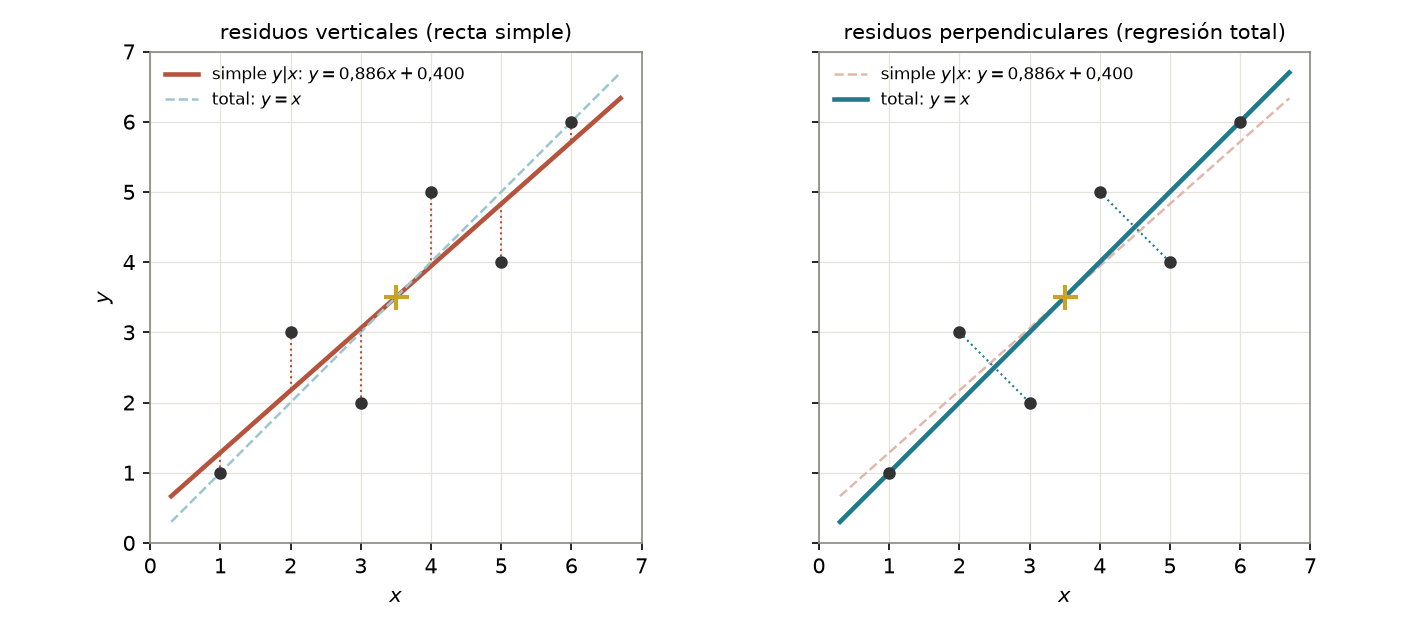
\includegraphics[width=.95\linewidth]{figuras/cuatro-problemas/cp_rectas.png}
\caption{Los seis puntos del ejemplo~\ref{ej:cp-rectas}. A la izquierda, la recta simple
\(y=0{,}886x+0{,}4\) con los residuos verticales que minimiza; a la derecha, la regresión
total \(y=x\) con los residuos perpendiculares. Las dos pasan por el baricentro (cruz). En
cada panel la otra recta aparece de trazos. Generada con
\texttt{apunte/scripts/cap12\_cuatro\_problemas.py}.}
\label{fig:cp-rectas}
\end{figure}

\subsection{Ajuste de un círculo}\label{sec:cuatro-problemas-circulo}

Imaginá que tenés que ubicar el centro y el radio de una rotonda a la que no se puede entrar
por el tránsito: solo se pueden marcar puntos sobre el cordón. Tres puntos determinan un
círculo, pero con nueve cada terna da un círculo un poco distinto. ¿Cuál pasa mejor por
todos? La misma pregunta aparece con cualquier cosa redonda que no se puede medir desde
adentro: un tanque, la base de una columna, una curva de un camino.

Buscar el círculo \((x-a)^2+(y-b)^2=r^2\), de centro \((a,b)\) y radio \(r\), que mejor pasa
por \(n\ge4\) puntos no es un problema lineal en \((a,b,r)\), porque los tres parámetros
aparecen elevados al cuadrado; pero un cambio de parámetros lo vuelve lineal.

\paragraph{Círculo algebraico.} Desarrollando los cuadrados,
\[
  x^2+y^2+Dx+Ey+F=0,\qquad D=-2a,\quad E=-2b,\quad F=a^2+b^2-r^2 .
\]
Los números \(D\), \(E\), \(F\) no tienen un significado geométrico directo; su ventaja es que
aparecen en forma lineal: cada punto da una ecuación
\(Dx_i+Ey_i+F=-(x_i^2+y_i^2)\), y con más de tres puntos se resuelve por mínimos cuadrados,
con matriz de columnas \((x_i)\), \((y_i)\), \((1)\). De la solución salen \(a=-\tfrac D2\),
\(b=-\tfrac E2\) y \(r=\sqrt{a^2+b^2-F}\).
Es la misma idea de los parámetros \(a=\lambda\cos\theta\), \(b=\lambda\sin\theta\) de la
transformación de Helmert, la similaridad que lleva coordenadas medidas con ejes propios al
sistema oficial (sección~\ref{sec:aplicacion-helmert}): elegir parámetros en los que el modelo
es lineal y recuperar los geométricos al final.

¿Qué se achica, en realidad, con ese atajo? No la distancia de cada punto al círculo, sino el
número \(x_i^2+y_i^2+Dx_i+Ey_i+F\), que llamamos \emph{residuo algebraico}. La proposición
siguiente dice cuánto se parece a una distancia.

\begin{proposicion}[Qué mide el residuo algebraico]\label{prop:cp-residuo-algebraico}
Si \(d_i=\lVert p_i-(a,b)\rVert\) es la distancia del punto al centro, el residuo
algebraico es
\[
  x_i^2+y_i^2+Dx_i+Ey_i+F=d_i^2-r^2=(d_i-r)(d_i+r)\approx 2r\,(d_i-r),
\]
donde la aproximación vale cuando \(d_i-r\) es chico frente a \(r\).
\end{proposicion}

\begin{demostracion}
Reemplazando \(D\), \(E\), \(F\):
\(x_i^2+y_i^2-2ax_i-2by_i+a^2+b^2-r^2=(x_i-a)^2+(y_i-b)^2-r^2=d_i^2-r^2\). Si
\(d_i=r+\varepsilon\), \(d_i+r=2r+\varepsilon\approx2r\).
\end{demostracion}

El círculo algebraico minimiza entonces, aproximadamente, \(4r^2\sum_i(d_i-r)^2\): la suma de
cuadrados de las distancias radiales, salvo un factor. La aproximación es buena cuando los
puntos quedan cerca del círculo; cuando no lo son, el círculo algebraico pesa más los puntos que quedan
afuera (\(d_i+r\) mayor) y tiende a subestimar el radio si los puntos cubren solo un arco
corto.

\paragraph{Círculo geométrico.} Lo que de verdad queremos achicar es la distancia de cada punto
al círculo, medida sobre el radio: cuánto queda el punto afuera (positivo) o adentro
(negativo). El criterio geométrico minimiza
\(\sum_if_i^2\) con \(f_i=d_i-r\), el residuo radial: la distancia de cada punto al
círculo, medida sobre el radio. El modelo ya no es un subespacio: al variar \((a,b,r)\), el
vector \((f_1,\dots,f_n)\) recorre un conjunto curvo.

Lo resolvemos linealizando: partimos de una estimación, reemplazamos el problema curvo por su
aproximación lineal cerca de ella, lo resolvemos, corregimos y
repetimos. Para eso hace falta saber cuánto cambia cada \(f_i\) si movemos un poco el centro o
el radio. Esa información es la matriz \(J\), la jacobiana del capítulo~\ref{cap:derivada}:
tiene una fila por punto y una columna por parámetro. En una estimación \((a,b,r)\), la
derivada de \(f_i\) respecto de los tres parámetros es la fila
\[
  J_i=\Big(-\frac{x_i-a}{d_i},\ -\frac{y_i-b}{d_i},\ -1\Big),
\]
o sea, menos el versor radial del punto y un \(-1\) para el radio. La corrección \(\delta\) de
los tres parámetros, el paso de Gauss--Newton, es la solución por mínimos cuadrados de
\(J\delta=-f\), con ecuaciones normales
\(J^TJ\,\delta=-J^Tf\): el método de Newton de la sección~\ref{sec:newton}, con más
ecuaciones que incógnitas. El círculo algebraico es un buen punto de partida, y una o dos
iteraciones alcanzan en los casos de campo.

\begin{proposicion}[El residuo radial en el óptimo]\label{prop:cp-circulo-optimo}
En el óptimo del ajuste geométrico, \(J^Tf=0\). Leída columna por columna: los residuos
radiales suman cero, \(\sum_if_i=0\), y \(\sum_if_i\,u_i=0\), donde \(u_i\) es el versor
radial del punto \(i\).
\end{proposicion}

\begin{demostracion}
La derivada de \(\tfrac12\sum_if_i^2\) respecto de los parámetros es \(J^Tf\), y en un mínimo
se anula. La tercera columna de \(J\) es \(-\mathbf 1\), y las dos primeras forman
\(-u_i^T\) en cada fila.
\end{demostracion}

El versor radial \(u_i\) es el vector de largo \(1\) que va del centro hacia el punto \(i\).
Imaginá cada residuo como un elástico que une el punto con el círculo a lo largo del radio y
tira con una fuerza proporcional a su largo. Hecho geométrico: \(\sum_if_i=0\) dice que el
radio que resulta es el promedio de las distancias al centro (los elásticos no consiguen agrandar
ni achicar el círculo); \(\sum_if_iu_i=0\) dice que los residuos radiales, vistos como
vectores, se equilibran: no queda ninguna dirección hacia la que convenga correr el centro.

\begin{ejemplo}[Círculo por siete puntos de un arco]\label{ej:cp-circulo}
El script genera siete puntos (semilla fija) cerca del círculo de centro \((3,2)\) y radio
\(5\), sobre un arco de \(210^\circ\), y los redondea a dos decimales:
\[
  (7{,}63;\ 0{,}30),\ (7{,}69;\ 3{,}26),\ (6{,}01;\ 5{,}83),\ (3{,}65;\ 6{,}73),\
  (0{,}52;\ 6{,}43),\ (-1{,}69;\ 4{,}00),\ (-1{,}85;\ 0{,}92).
\]
El círculo algebraico tiene \(D=-5{,}8097\), \(E=-3{,}9233\), \(F=-12{,}3116\), de donde
\[
  (a,b)=(2{,}9049;\ 1{,}9616),\qquad r=\sqrt{2{,}9049^2+1{,}9616^2+12{,}3116}=4{,}9596 .
\]
Los residuos algebraicos \(d_i^2-r^2\) valen
\((0{,}490;\ -0{,}015;\ 0{,}008;\ -1{,}305;\ 1{,}056;\ 0{,}670;\ -0{,}904)\) y son
perpendiculares a las tres columnas. Los residuos
radiales correspondientes, \(d_i-r\), suman \(-0{,}0045\): no cero, porque el círculo
algebraico no minimiza esas distancias.

Una iteración de Gauss--Newton desde el círculo algebraico resuelve
\[
  J^TJ=\begin{pmatrix}4{,}2485&0{,}0034&0{,}3271\\0{,}0034&2{,}7515&2{,}7717\\
  0{,}3271&2{,}7717&7\end{pmatrix},\qquad
  J^Tf=\begin{pmatrix}-0{,}0038\\0{,}0080\\0{,}0045\end{pmatrix},
\]
con paso \(\delta=(0{,}0008;\ -0{,}0037;\ 0{,}0008)\). El resultado,
\((a,b)=(2{,}9057;\ 1{,}9579)\) y \(r=4{,}9604\), coincide a cuatro decimales con el valor
al que convergen las iteraciones (seis, deteniéndolas cuando la corrección baja de
\(10^{-12}\)). Los residuos radiales
finales son \((0{,}046;\ -0{,}002;\ 0{,}002;\ -0{,}131;\ 0{,}108;\ 0{,}069;\ -0{,}093)\),
con suma de cuadrados \(0{,}044243\) (menor que la del círculo algebraico, \(0{,}044273\)),
suma cero y \(J^Tf=0\) a la precisión de la máquina (figura~\ref{fig:cp-circulo}).
\end{ejemplo}

\begin{figure}[htbp]
\centering
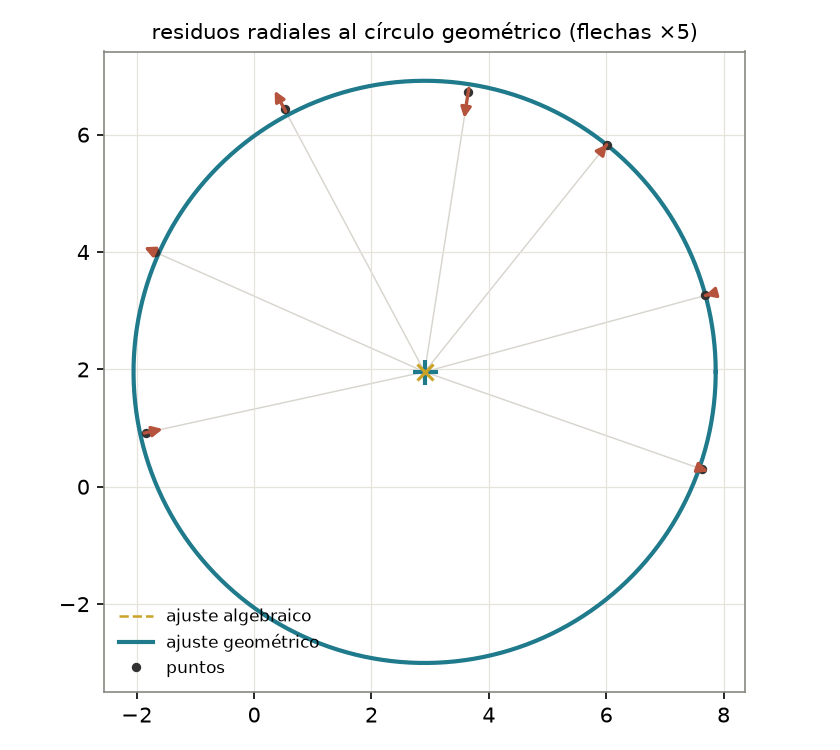
\includegraphics[width=.6\linewidth]{figuras/cuatro-problemas/cp_circulo.png}
\caption{El círculo geométrico del ejemplo~\ref{ej:cp-circulo} y los residuos radiales de los
siete puntos, dibujados sobre cada radio y multiplicados por \(5\) para que se vean. El
círculo algebraico (de trazos) se aparta del geométrico menos de \(0{,}004\) en el centro
y en el radio, y a esta escala queda tapado. Generada con
\texttt{apunte/scripts/cap12\_cuatro\_problemas.py}.}
\label{fig:cp-circulo}
\end{figure}

\subsection{Procrustes ortogonal}\label{sec:cuatro-problemas-procrustes}

Imaginá dos calcos del mismo terreno, dibujados por dos personas que eligieron ejes distintos
y, quizás, unidades apenas distintas. Ponés uno encima del otro a contraluz y lo girás y lo
corrés, sin deformarlo, hasta que los vértices coincidan lo mejor posible. ¿Cuánto hay que
girar y cuánto correr? Responderlo con números sirve para pasar una medición hecha con ejes
propios al sistema oficial, o para comparar dos mediciones del mismo terreno y descubrir si
algún vértice se movió.

Dos nubes homólogas \(a_1,\dots,a_n\) y \(b_1,\dots,b_n\) son el mismo conjunto de puntos
medido en dos sistemas: el punto \(a_i\) de una corresponde al \(b_i\) de la otra. Buscamos
la rotación \(R\) (ortogonal, con \(\det R=+1\)), la traslación \(t\), que es el corrimiento,
y, si corresponde, la escala \(s>0\), el factor que estira o encoge, que mejor llevan una nube
sobre la otra:
\[
  \min\ \sum_i\lVert b_i-(sRa_i+t)\rVert^2 .
\]
El nombre viene del posadero de la mitología griega que estiraba o recortaba a sus huéspedes
para que cupieran en la cama; acá solo se permite mover y, a lo sumo, escalar.

\paragraph{Primero, centrar.} Con los calcos, lo primero que uno hace es superponer los centros
de los dos dibujos y recién después girar. La cuenta dice lo mismo. Para \(s\) y \(R\) fijos,
la derivada respecto de \(t\) da
\(\sum_i\big(b_i-sRa_i-t\big)=0\): los residuos suman cero y \(t=\bar b-sR\,\bar a\), el
baricentro de una nube va al baricentro de la otra. Con las nubes centradas,
\(a_i'=a_i-\bar a\), \(b_i'=b_i-\bar b\), el problema queda sin traslación:
\(\min\sum_i\lVert b_i'-sRa_i'\rVert^2\). Desarrollando el cuadrado y usando que \(R\)
conserva las normas,
\[
  \sum_i\lVert b_i'-sRa_i'\rVert^2=\sum_i\lVert b_i'\rVert^2+s^2\sum_i\lVert a_i'\rVert^2
  -2s\sum_i b_i'^{\,T}Ra_i',
\]
y minimizar es maximizar \(\sum_ib_i'^{\,T}Ra_i'=\operatorname{tr}(RM^T)\), con
\(M=B_0^TA_0=\sum_i b_i'\,a_i'^{\,T}\), donde \(A_0\) y \(B_0\) son las matrices de \(n\times2\) de las nubes centradas, un punto por
fila. (La igualdad sale de \(b^TRa=\operatorname{tr}(Rab^T)\).) La traza \(\operatorname{tr}\)
es la suma de la diagonal, y la matriz \(M\), de \(2\times2\), resume cómo se corresponden las
dos nubes: es lo único de los datos que necesita la rotación.

Para hallar la rotación usamos la descomposición en valores singulares de \(M\),
\(M=U\Sigma V^T\): \(U\) y \(V\) son matrices ortogonales (rotaciones o reflexiones) y
\(\Sigma\) es diagonal, con los valores singulares \(\sigma_1\ge\sigma_2\) de \(M\).

\begin{proposicion}[Rotación óptima de Procrustes]\label{prop:cp-procrustes}
Sea \(M=B_0^TA_0=U\Sigma V^T\) su SVD, con \(\sigma_1\ge\sigma_2\ge0\). La rotación que
maximiza \(\operatorname{tr}(RM^T)\) es
\[
  \boxed{\ R=U\begin{pmatrix}1&0\\0&\det(UV^T)\end{pmatrix}V^T\ } ,
\]
que se reduce a \(R=UV^T\) cuando \(\det(UV^T)=+1\). La escala óptima es
\(s=\big(\sigma_1+\det(UV^T)\,\sigma_2\big)\big/\sum_i\lVert a_i'\rVert^2\) y la traslación,
\(t=\bar b-sR\bar a\).
\end{proposicion}

La demostración, que separa el caso en que \(UV^T\) es una rotación del caso en que es una
reflexión, está en la sección~\ref{sec:cp-demostraciones}.

La corrección del determinante no es un detalle: sin ella, la SVD puede devolver una
reflexión, que lleva una nube sobre la otra \enquote{dada vuelta}, como un calco puesto del
revés. Si los datos fueron tomados con ejes en espejo (por ejemplo, con un eje invertido por
error al cargar una planilla), la reflexión calza mejor, y el valor \(\det(UV^T)=-1\) es la
alarma (ejercicio~\ref{ex:cp-reflexion}).

\begin{ejemplo}[Procrustes con cuatro puntos]\label{ej:cp-procrustes}
La nube \(A\) tiene los puntos \((0,0)\), \((4,0)\), \((4,2)\), \((0,3)\). La nube \(B\) se
obtuvo girándola \(30^\circ\), trasladándola \((6,1)\), agregando perturbaciones de algunos
centímetros (de \(0{,}02\) a \(0{,}06\)) y redondeando a dos decimales:
\[
  b_1=(6{,}05;\ 0{,}96),\quad b_2=(9{,}43;\ 3{,}06),\quad b_3=(8{,}50;\ 4{,}75),\quad
  b_4=(4{,}44;\ 3{,}56).
\]
Los baricentros son \(\bar a=(2;\ 1{,}25)\) y \(\bar b=(7{,}105;\ 3{,}0825)\), y
\[
  M=B_0^TA_0=\begin{pmatrix}14{,}88&-5{,}205\\6{,}58&4{,}7675\end{pmatrix},\qquad
  \sigma_1=16{,}5582,\quad \sigma_2=6{,}3527,\quad \det(UV^T)=+1 .
\]
No hace falta corrección, y
\[
  R=UV^T=\begin{pmatrix}0{,}8576&-0{,}5144\\0{,}5144&0{,}8576\end{pmatrix},
  \qquad \theta=30{,}956^\circ,\qquad \det R=1,\qquad t=\bar b-R\bar a=(6{,}0329;\ 0{,}9818).
\]
Los residuos \(b_i-(Ra_i+t)\) son \((0{,}017;\ -0{,}022)\), \((-0{,}033;\ 0{,}021)\),
\((0{,}066;\ -0{,}004)\), \((-0{,}050;\ 0{,}006)\): suman \((0,0)\) y la suma de sus
cuadrados es \(0{,}009125\). Con escala libre, \(s=1{,}0071\), el mismo giro y una suma de
cuadrados de \(0{,}007987\). El giro recuperado se aparta casi un grado de los \(30^\circ\)
con que se generó \(B\) porque las perturbaciones, de varios centímetros sobre una nube de
cuatro unidades, son grandes en proporción (figura~\ref{fig:cp-procrustes}).
\end{ejemplo}

\begin{figure}[htbp]
\centering
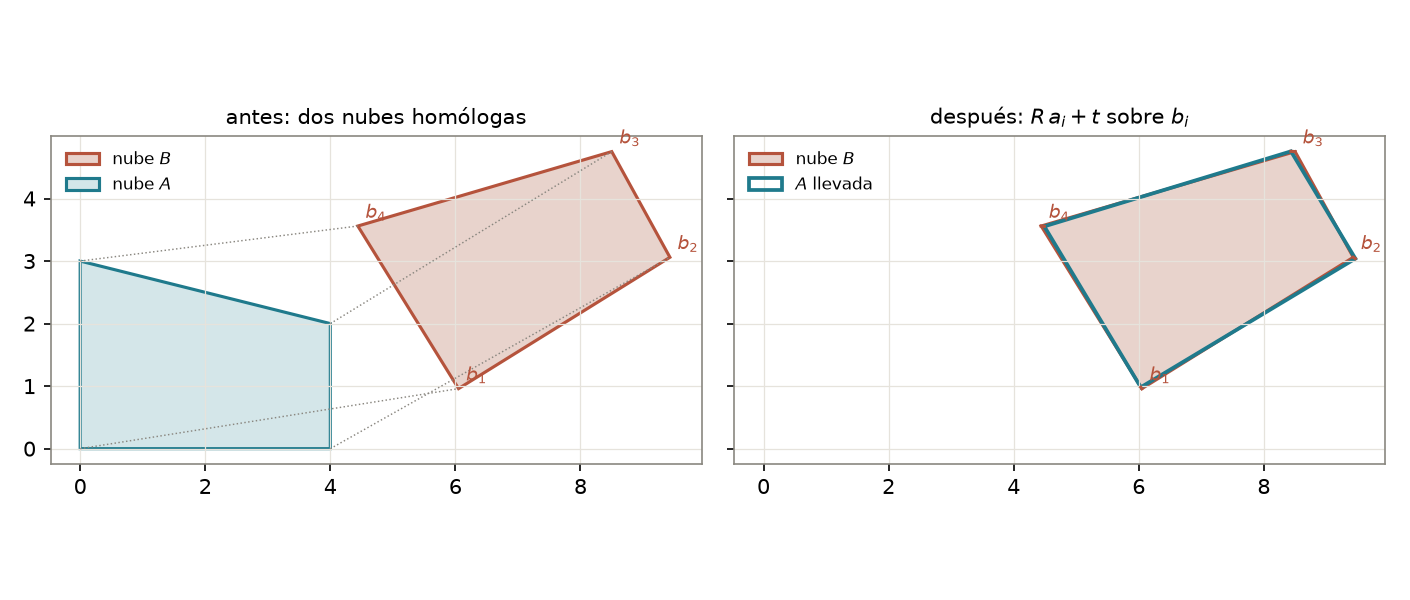
\includegraphics[width=.95\linewidth]{figuras/cuatro-problemas/cp_procrustes.png}
\caption{Las dos nubes del ejemplo~\ref{ej:cp-procrustes}. Antes: la nube \(A\) en su
sistema y la \(B\), con las líneas punteadas que unen puntos homólogos. Después: \(A\)
llevada por la rotación y la traslación óptimas cae sobre \(B\); los residuos, de algunos
centímetros, son los segmentos que todavía separan cada par. Generada con
\texttt{apunte/scripts/cap12\_cuatro\_problemas.py}.}
\label{fig:cp-procrustes}
\end{figure}

\subsection{Simulaciones}

\unidadInteractiva{11_cuatro_problemas}{Cuatro problemas: regresión, círculos, Procrustes, regresión total}{Verificá: en el problema «(c) Procrustes: dos relevamientos del mismo lote» poné el ruido del segundo relevamiento en \(0\) y comprobá que los números vivos devuelven el giro de \(25^\circ\), la escala \(1{,}2\) y la traslación \((1{,}5;\ 0{,}5)\). Después subí el ruido y verificá que la comprobación \(\sum_i\langle r_i,Rp_{0i}\rangle\) sigue dando \(0\).}

\unidadInteractiva{11_cuatro_problemas}{Cuatro problemas: regresión, círculos, Procrustes, regresión total}{Verificá: en el problema «(a) recta de ajuste» mové el ruido en \(y\) y comprobá que \(A^Tr\) sigue dando \((0,0)\); después pasá a «(d) regresión total» y verificá que la suma de los cuadrados de las distancias perpendiculares coincide con el autovalor menor de \(C\).}

\section{En profundidad}

\subsection{Una sola geometría}

Volvamos a la pregunta de \enquote{La idea}: si nada pasa por todos los puntos, ¿qué pasa más cerca?
El cuadro reúne las cuatro respuestas.

{\small
\begin{center}
\begin{tabularx}{\textwidth}{>{\bfseries}p{24mm} Y Y Y}
\toprule
Problema & Lo que el modelo puede producir & Residuo & Cómo se resuelve\\
\midrule
Recta simple & plano \(\operatorname{im}A\) de \(\R^n\) (columnas \(x\) y \(\mathbf 1\)) &
vertical & ecuaciones normales\\
Regresión total & nubes alineadas: conjunto curvo en \(\R^{2n}\) &
perpendicular a la recta & autovector de \(\Sigma_0\) (SVD)\\
Círculo & algebraico: subespacio en \((D,E,F)\); geométrico: conjunto curvo &
radial & lineal, luego Gauss--Newton\\
Procrustes & copias movidas de una nube: órbita de las rotaciones &
punto a punto & SVD de \(B_0^TA_0\)\\
\bottomrule
\end{tabularx}
\end{center}
}

En los cuatro, la condición de óptimo es una perpendicularidad. En la recta simple y en el
círculo algebraico, el residuo es perpendicular al subespacio del modelo (\(A^Tr=0\)). En
los otros dos casos, el modelo es curvo y el residuo resulta perpendicular al plano tangente
en el punto más cercano: \(J^Tf=0\) en el círculo geométrico; en la regresión total,
\(\sum_i(d\cdot(p_i-\bar p))(n\cdot(p_i-\bar p))=d^T\Sigma_0n=0\), que dice que los residuos no
tienen correlación con el avance sobre la recta (girar la recta un poco no los achica); en
Procrustes, \(\sum_ir_i=0\) (trasladar no mejora) y
\(\sum_ir_i\times Ra_i'=0\) (girar un poco no mejora).

La diferencia práctica entre modelos lineales y curvos es que los primeros se resuelven en
un paso y los segundos necesitan una idea más: la SVD, cuando la curvatura es la de las
rotaciones o la de las direcciones (regresión total, Procrustes), o la linealización
iterada, en los demás casos. El mismo Gauss--Newton resuelve la intersección de
circunferencias del capítulo~\ref{cap:derivada}: allí los centros son puntos de coordenadas
conocidas y solo el punto buscado es incógnita, con la fila \(J_i=-u_i^T\) de la sección
anterior sin la columna del radio.

\subsection{Procrustes y Helmert}

La transformación de Helmert de la sección~\ref{sec:aplicacion-helmert} es una similaridad
\(q=sR(\theta)p+t\), escrita con los parámetros lineales \(a=s\cos\theta\),
\(b=s\sin\theta\). Para fijarla se usan puntos de control, puntos cuyas coordenadas se conocen
en los dos sistemas. Con dos puntos de control, la solución es exacta; con tres o más, el
sistema es incompatible y se resuelve por mínimos cuadrados. Procrustes con escala resuelve
el mismo problema por otro camino, y los dos coinciden.

\begin{proposicion}[Procrustes en el plano]\label{prop:cp-procrustes-helmert}
Con las nubes centradas \(p_i=a_i-\bar a\), \(q_i=b_i-\bar b\), sean
\(P=\sum_ip_i\cdot q_i\) y \(Q=\sum_ip_i\times q_i\), donde
\(p\times q=p_xq_y-p_yq_x\) es el producto cuña. La rotación y la escala de Procrustes son
\[
  \theta=\operatorname{atan2}(Q,P),\qquad s=\frac{\sqrt{P^2+Q^2}}{\sum_i\lVert p_i\rVert^2},
\]
y coinciden con las del ajuste de Helmert por mínimos cuadrados:
\(a=P/\sum_i\lVert p_i\rVert^2\), \(b=Q/\sum_i\lVert p_i\rVert^2\).
\end{proposicion}

\begin{demostracion}
Con \(M=B_0^TA_0\), \(M_{11}+M_{22}=\sum_i(q_{ix}p_{ix}+q_{iy}p_{iy})=P\) y
\(M_{21}-M_{12}=\sum_i(q_{iy}p_{ix}-q_{ix}p_{iy})=Q\). Para
\(R=\left(\begin{smallmatrix}\cos\theta&-\sin\theta\\\sin\theta&\cos\theta\end{smallmatrix}\right)\),
\(\operatorname{tr}(RM^T)=\sum_{jk}R_{jk}M_{jk}=P\cos\theta+Q\sin\theta\), que es máximo
cuando \((\cos\theta,\sin\theta)\) apunta como \((P,Q)\), con valor \(\sqrt{P^2+Q^2}\). La
escala sale de la proposición~\ref{prop:cp-procrustes}. Las ecuaciones normales del
ajuste de Helmert con coordenadas centradas dan \(a\) y \(b\)
(ejercicio~\ref{ex:cp-helmert}), y \((a,b)=s(\cos\theta,\sin\theta)\).
\end{demostracion}

En el plano, entonces, la rotación de Procrustes sale con un \(\operatorname{atan2}\) y es
siempre una rotación: el problema del determinante solo aparece al usar la SVD, y en el
espacio, donde la rotación no se puede escribir con parámetros lineales. Allí Procrustes es
la manera directa de resolver por mínimos cuadrados el mismo modelo de la similaridad.

\paragraph{Los tres puntos de control de Helmert.} La sección~\ref{sec:aplicacion-helmert}
terminó con tres puntos de control, \(C_1\), \(C_2\), \(C_3\), que ninguna similaridad
satisface a la vez, y dejó planteado el reparto de la discrepancia. Con los datos de esa
sección (coordenadas oficiales reducidas a su baricentro, \(E=5\,432\,175{,}305\),
\(N=6\,154\,500{,}022\); los números son largos porque el origen oficial está lejos, y lo que
importa son las diferencias entre puntos), Procrustes con escala da
\[
  s=1{,}0000751,\qquad \theta=27{,}85114^\circ,\qquad
  t=(5\,432\,100{,}017;\ 6\,154\,300{,}002),
\]
y el ajuste lineal de Helmert por mínimos cuadrados, con incógnitas \((a,b,t_E,t_N)\), da
\(a=0{,}8842307\), \(b=0{,}4672110\), los mismos \(s\) y \(\theta\) (la diferencia es del
orden de \(10^{-16}\)) y la misma suma de cuadrados de residuos, \(0{,}000665\) m\(^2\). Los
residuos en los tres puntos son \((-0{,}013;\ 0{,}001)\), \((0{,}004;\ 0{,}014)\) y
\((0{,}009;\ -0{,}015)\) m: suman cero, y el residuo medio por punto es de \(0{,}015\) m. La
escala queda entre las que daban los pares de puntos (\(1{,}0001479\) con \(C_1C_2\),
\(0{,}9999984\) con \(C_1C_3\)), y la discrepancia de \(0{,}039\) m que concentraba \(C_3\)
se reparte entre los tres.

\subsection{Aplicación topográfica: eje de una medianera, una rotonda y dos levantamientos}

Volvemos a las tres situaciones de \enquote{La idea}, ahora con números de terreno: trazar el eje de
una pared con diez puntos, ubicar el centro de una rotonda con nueve puntos del cordón y
comparar dos mediciones del mismo terreno hechas con años de diferencia.

\begin{idea}[Esto lo vas a usar en Topografía]
Las coordenadas de esta sección están en el sistema plano oficial del país, llamado
Gauss-Krüger: \(E\) crece hacia el este y \(N\) hacia el norte, en metros, y el país se divide
en franjas norte-sur (las \emph{fajas}) para poder dibujarlo en un plano; acá todo está en la
faja~5. Los números tienen siete cifras porque el origen del sistema está muy lejos; importan
las diferencias entre puntos, que son de algunas decenas de metros. La dirección de una recta
se da con el \emph{acimut}, el ángulo que forma con el norte contado en sentido horario.
\end{idea}

Escritas \((E,N)\) como en la caja de la sección~\ref{caja:convencion-en}, las coordenadas
completas tienen siete cifras enteras, y elevarlas al cuadrado (como pide el círculo
algebraico) o multiplicarlas entre sí pierde cifras significativas en doble precisión; por eso
todas las cuentas se hacen con coordenadas reducidas al baricentro de cada nube, y los
resultados se vuelven a expresar en coordenadas completas al final. Los datos son sintéticos:
los generó el script con semilla fija, con errores de algunos centímetros.

\paragraph{1. El eje de una medianera.} Hay que trazar el eje de una pared medianera de unos
\(18\) m. Con un receptor satelital, un aparato que calcula su posición con las señales de los
satélites con un error de pocos centímetros, se tomaron diez puntos sobre la pared, con un
error de unos \(3\) cm en cada coordenada:
\begin{center}
\small
\begin{tabular}{crr@{\qquad}crr}
\toprule
punto & \(E\) (m) & \(N\) (m) & punto & \(E\) (m) & \(N\) (m)\\
\midrule
1 & \(5\,434\,512{,}029\) & \(6\,152\,845{,}982\) & 6 & \(5\,434\,518{,}634\) & \(6\,152\,853{,}535\)\\
2 & \(5\,434\,513{,}341\) & \(6\,152\,847{,}514\) & 7 & \(5\,434\,519{,}958\) & \(6\,152\,854{,}968\)\\
3 & \(5\,434\,514{,}645\) & \(6\,152\,849{,}008\) & 8 & \(5\,434\,521{,}281\) & \(6\,152\,856{,}473\)\\
4 & \(5\,434\,515{,}921\) & \(6\,152\,850{,}528\) & 9 & \(5\,434\,522{,}627\) & \(6\,152\,857{,}997\)\\
5 & \(5\,434\,517{,}301\) & \(6\,152\,851{,}988\) & 10 & \(5\,434\,523{,}888\) & \(6\,152\,859{,}503\)\\
\bottomrule
\end{tabular}
\end{center}
El baricentro es \((5\,434\,517{,}963;\ 6\,152\,852{,}750)\), y con las coordenadas reducidas
\(S_{EE}=144{,}4903\), \(S_{NN}=185{,}2725\), \(S_{EN}=163{,}6079\) m\(^2\). El acimut de una
recta se mide desde el norte en sentido horario: si la recta avanza \(\Delta E\) al este por
cada \(\Delta N\) al norte, su acimut es \(\operatorname{atan2}(\Delta E,\Delta N)\).
\begin{itemize}
  \item Recta de \(N\) sobre \(E\) (distancias medidas en \(N\)): \(dN/dE=S_{EN}/S_{EE}=1{,}132311\),
  acimut \(41^\circ26'57{,}6''\).
  \item Recta de \(E\) sobre \(N\) (distancias medidas en \(E\)): \(dE/dN=S_{EN}/S_{NN}=0{,}883066\),
  acimut \(41^\circ26'47{,}9''\).
  \item Regresión total: \(d=v_1=(0{,}6619;\ 0{,}7496)\), con valores singulares
  \(\sigma_1=18{,}159\) m y \(\sigma_2=0{,}0875\) m; acimut \(41^\circ26'52{,}1''\).
\end{itemize}
Las dos regresiones simples se apartan de la total \(+5{,}4''\) y \(-4{,}2''\), y entre sí
\(9{,}7''\), y la total queda en el medio, como corresponde a la
proposición~\ref{prop:cp-total-entre}. Verificaciones: los residuos de la recta \(N\) sobre \(E\) suman cero y son
perpendiculares a la columna de las \(E\) reducidas; las distancias perpendiculares a la
recta total suman cero, tienen un valor cuadrático medio de \(2{,}77\) cm y cumplen
\(d^T\Sigma_0n=0\). El script gira además los ejes \(30^\circ\) y repite las cuentas: la dirección de
la regresión simple cambia \(18{,}2''\) respecto de la medianera, y la de la total no cambia
(diferencia del orden de \(10^{-11}\) segundos).

Por qué la total es la correcta acá: el error está en las dos coordenadas y con la misma
precisión, de modo que no hay un eje privilegiado. La regresión simple supone que una
coordenada es exacta, y la respuesta depende de cuál se elija y de cómo estén orientados los
ejes; la total minimiza distancias, que no dependen de los ejes. Conviene leer las magnitudes con
cuidado. Llamamos \(\sigma_0\) al error típico de un punto, estimado con los mismos datos:
\(\sigma_0=\sigma_2/\sqrt{n-2}=3{,}09\) cm. Con una base de \(18\) m y \(3\) cm de error, la
incertidumbre típica (el desvío) de la dirección del eje es de unos
\(\sigma_0/\sigma_1\approx351''\), de modo que
la diferencia entre métodos (segundos) es chica frente a la incertidumbre del eje (minutos).
El eje se generó con acimut \(41^\circ30'\), y la total lo recupera con una diferencia de
\(188''\), dentro de ese desvío. Lo que hace inaceptable a la regresión simple no es el
tamaño de su diferencia, sino que es sistemática y depende de una elección arbitraria.

\paragraph{2. El centro y el radio de una rotonda.} Hay que ubicar el centro y el radio de
una rotonda. Del cordón se marcaron nueve puntos sobre la mitad sur, de este a oeste (el resto
quedaba tapado por el tránsito):
\begin{center}
\small
\begin{tabular}{crr@{\qquad}crr}
\toprule
punto & \(E\) (m) & \(N\) (m) & punto & \(E\) (m) & \(N\) (m)\\
\midrule
1 & \(5\,434\,668{,}761\) & \(6\,152\,928{,}538\) & 6 & \(5\,434\,647{,}406\) & \(6\,152\,919{,}271\)\\
2 & \(5\,434\,666{,}819\) & \(6\,152\,923{,}604\) & 7 & \(5\,434\,643{,}427\) & \(6\,152\,923{,}188\)\\
3 & \(5\,434\,663{,}026\) & \(6\,152\,919{,}547\) & 8 & \(5\,434\,641{,}300\) & \(6\,152\,928{,}084\)\\
4 & \(5\,434\,657{,}939\) & \(6\,152\,917{,}321\) & 9 & \(5\,434\,641{,}212\) & \(6\,152\,933{,}439\)\\
5 & \(5\,434\,652{,}566\) & \(6\,152\,917{,}208\) & & &\\
\bottomrule
\end{tabular}
\end{center}
Con coordenadas reducidas al baricentro \((5\,434\,653{,}606;\ 6\,152\,923{,}356)\), el círculo
algebraico tiene \(D=-2{,}7640\), \(E=-15{,}2909\), \(F=-135{,}1478\): centro reducido
\((1{,}3820;\ 7{,}6455)\) y radio \(13{,}9825\) m. Una iteración de Gauss--Newton lo corrige en
décimas de milímetro, y las siguientes (cuatro en total) ya no lo mueven. El resultado es
\[
  \boxed{\ E_c=5\,434\,654{,}988\ \text{m},\quad N_c=6\,152\,931{,}001\ \text{m},\quad r=13{,}983\ \text{m}\ } .
\]
Los residuos radiales, en centímetros, son
\[
  (0{,}87;\ -2{,}96;\ 1{,}04;\ 1{,}22;\ 2{,}16;\ -1{,}52;\ -2{,}88;\ 1{,}31;\ 0{,}77),
\]
con valor cuadrático medio \(1{,}82\) cm y máximo \(2{,}96\) cm (figura~\ref{fig:cp-rotonda}).
Verificaciones: suman cero y \(J^Tf=0\) (proposición~\ref{prop:cp-circulo-optimo}); el
residuo algebraico es perpendicular a las tres columnas. Con \(\sigma_0=2{,}23\) cm, el error
típico de un punto estimado con las \(9-3=6\) mediciones de más (los grados de libertad), y
con \((J^TJ)^{-1}\), que dice cómo pasan los errores de las mediciones al centro y al radio,
los desvíos estimados del centro son
\(1{,}04\) cm en \(E\) y \(2{,}01\) cm en \(N\), y el del radio, \(1{,}35\) cm. Que el desvío
en \(N\) duplique al de \(E\) es geometría: los puntos marcados están casi todos al sur del
centro, y el norte del círculo no aporta. Con errores de centímetros sobre un radio de
\(14\) m, el círculo algebraico y el geométrico coinciden a la décima de milímetro: la
aproximación \(d_i^2-r^2\approx2r(d_i-r)\) es excelente. La rotonda se generó con radio
\(14{,}000\) m; el resultado da \(13{,}983\) m, a poco más de un desvío.

\begin{figure}[htbp]
\centering
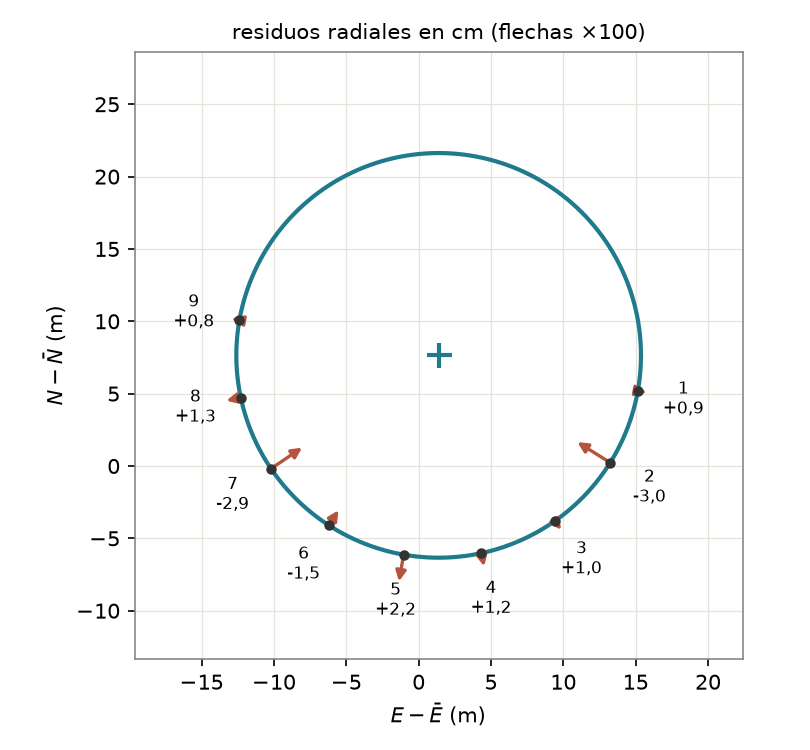
\includegraphics[width=.6\linewidth]{figuras/cuatro-problemas/cp_rotonda.png}
\caption{La rotonda en coordenadas reducidas al baricentro de los puntos relevados. Cada
flecha es el residuo radial de un punto, multiplicado por \(100\); el número es el residuo en
centímetros (positivo: el punto está afuera del círculo). Generada con
\texttt{apunte/scripts/cap12\_cuatro\_problemas.py}.}
\label{fig:cp-rotonda}
\end{figure}

\paragraph{3. Dos levantamientos del mismo predio.} Un predio de seis vértices se midió dos
veces. La primera vez, en el sistema oficial (levantamiento 1); años después, con un
instrumento que mide ángulos y distancias desde un punto elegido a gusto, en ejes propios con
origen arbitrario (levantamiento 2). ¿Son compatibles las dos mediciones, o algún vértice se
movió? Para saberlo, llevamos una sobre la otra con la mejor similaridad y miramos lo que sobra:
\begin{center}
\small
\begin{tabular}{crrrr}
\toprule
vértice & \(E\) (m) & \(N\) (m) & \(x\) (m) & \(y\) (m)\\
\midrule
\(V_1\) & \(5\,434\,720{,}412\) & \(6\,153\,018{,}237\) & \(1034{,}451\) & \(1023{,}451\)\\
\(V_2\) & \(5\,434\,748{,}905\) & \(6\,153\,041{,}118\) & \(1067{,}698\) & \(1008{,}319\)\\
\(V_3\) & \(5\,434\,771{,}364\) & \(6\,153\,013{,}552\) & \(1053{,}196\) & \(975{,}845\)\\
\(V_4\) & \(5\,434\,766{,}020\) & \(6\,152\,982{,}774\) & \(1023{,}302\) & \(966{,}766\)\\
\(V_5\) & \(5\,434\,739{,}181\) & \(6\,152\,969{,}405\) & \(999{,}293\) & \(984{,}725\)\\
\(V_6\) & \(5\,434\,718{,}733\) & \(6\,152\,990{,}861\) & \(1009{,}248\) & \(1012{,}625\)\\
\bottomrule
\end{tabular}
\end{center}
Buscamos la similaridad que lleva el levantamiento 2 sobre el 1, \((E,N)=sR(x,y)+t\). Los
baricentros son \((5\,434\,744{,}103;\ 6\,153\,002{,}658)\) y \((1031{,}198;\ 995{,}289)\).
Con las nubes centradas, \(M\) tiene valores singulares \(3499{,}68\) y \(2456{,}33\) y
\(\det(UV^T)=+1\), y Procrustes da
\[
  \theta=63^\circ15'03{,}0'',\qquad s=1{,}000092\ (92\ \text{partes por millón}),\qquad
  t=(5\,435\,168{,}793;\ 6\,151\,633{,}722),
\]
con \(\det R=1{,}000000000000\). Los residuos, en centímetros, son
\begin{center}
\small
\begin{tabular}{lrrrrrr}
\toprule
& \(V_1\) & \(V_2\) & \(V_3\) & \(V_4\) & \(V_5\) & \(V_6\)\\
\midrule
\(r_E\) & \(-0{,}37\) & \(1{,}00\) & \(-0{,}47\) & \(-0{,}08\) & \(0{,}59\) & \(-0{,}66\)\\
\(r_N\) & \(-0{,}27\) & \(-0{,}22\) & \(0{,}05\) & \(0{,}66\) & \(-0{,}46\) & \(0{,}24\)\\
\(\lVert r\rVert\) & \(0{,}46\) & \(1{,}02\) & \(0{,}48\) & \(0{,}66\) & \(0{,}75\) & \(0{,}70\)\\
\bottomrule
\end{tabular}
\end{center}
y el RMS por punto (la raíz del promedio de los cuadrados, el mismo valor cuadrático medio de
antes) es de \(0{,}70\) cm (\(0{,}50\) cm por coordenada). Verificaciones: los
residuos suman \((0,0)\), \(\sum_ir_i\times sRa_i'=0\) y \(\det R=+1\). Sin escala, el giro es
el mismo y el RMS sube a \(0{,}76\) cm: las \(92\) partes por millón representan unos
\(3\) mm a \(30\) m, del orden de los residuos, de modo que la escala no
alcanza a distinguirse del error de medición (los vértices están, en promedio, a unos \(31\) m del
baricentro). Lectura de la comparación: ningún vértice se
aparta más de \(1{,}02\) cm de la similaridad, compatible con los errores de las dos
mediciones; una marca de vértice movida o confundida con otra aparecería como un residuo
varias veces mayor que el resto. Los datos se generaron con un giro de \(-63{,}25^\circ\) y una escala de
\(0{,}99988\) del levantamiento 1 al 2; la transformación inversa tiene giro
\(+63^\circ15'\) y escala \(1/0{,}99988=1{,}00012\), y la estimación difiere en
\(3''\) y en \(28\) partes por millón.

\subsection{Demostraciones de la regresión total y de Procrustes}\label{sec:cp-demostraciones}

\paragraph{Demostración de la proposición~\ref{prop:cp-total-entre}.} La idea es escribir la
condición de autovector como una ecuación de segundo grado en la pendiente y ubicar \(m\) y
\(1/m'\) respecto de sus raíces.

\begin{demostracion}
Sea \(v_1=(d_1,d_2)\). Si fuera \(d_1=0\), la primera fila de \(\Sigma_0v_1=\lambda_1v_1\) daría
\(S_{xy}d_2=0\), imposible; así que \(m_{\mathrm{tot}}=d_2/d_1\) existe. Las dos filas de
\(\Sigma_0v_1=\lambda_1v_1\) son \(S_{xx}d_1+S_{xy}d_2=\lambda_1d_1\) y
\(S_{xy}d_1+S_{yy}d_2=\lambda_1d_2\). Multiplicando la primera por \(d_2\), la segunda por
\(d_1\) e igualando, y dividiendo por \(d_1^2\),
\[
  p(m_{\mathrm{tot}})=0,\qquad p(z)=S_{xy}z^2+(S_{xx}-S_{yy})\,z-S_{xy} .
\]
Con \(S_{xy}>0\), \(p\) es una parábola que abre hacia arriba y el producto de sus raíces es
\(-1\): una raíz es negativa y la otra positiva. La pendiente \(m_{\mathrm{tot}}\) es la positiva, porque el
autovalor mayor supera a cada elemento de la diagonal cuando \(S_{xy}\neq0\):
\[
  \lambda_1=\frac{S_{xx}+S_{yy}}2+\sqrt{\Big(\frac{S_{xx}-S_{yy}}2\Big)^2+S_{xy}^2}
  >\frac{S_{xx}+S_{yy}}2+\frac{\lvert S_{xx}-S_{yy}\rvert}2=\max(S_{xx},S_{yy}),
\]
así que \(m_{\mathrm{tot}}=(\lambda_1-S_{xx})/S_{xy}>0\). Evaluando,
\[
  p(m)=\frac{S_{xy}}{S_{xx}^2}\,\big(S_{xy}^2-S_{xx}S_{yy}\big)<0,\qquad
  p\Big(\frac1{m'}\Big)=\frac{S_{xx}S_{yy}-S_{xy}^2}{S_{xy}}>0,
\]
por Cauchy--Schwarz estricta (proposición~\ref{prop:cp-dos-regresiones}). Como \(p(m)<0\),
\(m\) está entre las dos raíces, y por ser \(m>0\), \(m<m_{\mathrm{tot}}\). Como \(p(1/m')>0\) y
\(1/m'>0\), \(1/m'\) está a la derecha de las dos raíces: \(m_{\mathrm{tot}}<1/m'\). Si \(S_{xy}<0\), el
cambio \(y\mapsto-y\) cambia el signo de \(S_{xy}\), de \(m\), de \(1/m'\) y de \(m_{\mathrm{tot}}\), y da
las desigualdades invertidas.
\end{demostracion}

\paragraph{Demostración de la proposición~\ref{prop:cp-procrustes}.} La idea es pasar la
rotación buscada a las bases de la SVD, donde la traza se lee en la diagonal.

\begin{demostracion}
\(\operatorname{tr}(RM^T)=\operatorname{tr}(RV\Sigma U^T)=\operatorname{tr}(U^TRV\,\Sigma)
=\sigma_1z_{11}+\sigma_2z_{22}\), con \(Z=U^TRV\), que es ortogonal porque lo son \(U\), \(R\)
y \(V\). Las entradas de una matriz ortogonal no superan \(1\) en valor absoluto, así que
\(\operatorname{tr}(RM^T)\le\sigma_1+\sigma_2\), con igualdad si \(Z=I\), es decir,
\(R=UV^T\). Esa \(R\) es una rotación si \(\det(UV^T)=+1\). Si \(\det(UV^T)=-1\), toda
rotación \(R\) da \(\det Z=\det U\det V=-1\): \(Z\) es una reflexión,
\(Z=\left(\begin{smallmatrix}\cos\varphi&\sin\varphi\\\sin\varphi&-\cos\varphi\end{smallmatrix}\right)\),
y \(\sigma_1z_{11}+\sigma_2z_{22}=(\sigma_1-\sigma_2)\cos\varphi\), máximo en \(\varphi=0\):
\(Z=\operatorname{diag}(1,-1)\). En los dos casos el máximo vale
\(\sigma_1+\det(UV^T)\sigma_2\). Para \(R\) fija, la expresión de arriba es una parábola en
\(s\), con mínimo en \(s=\operatorname{tr}(RM^T)/\sum_i\lVert a_i'\rVert^2\).
\end{demostracion}

\section{Ejercicios con solución}

\begin{ejercicio}\label{ex:cp-dos-rectas}
Para los puntos \((0,0)\), \((1,1)\), \((2,1)\), \((3,4)\), calculá la recta de \(y\) sobre
\(x\), sus residuos y la suma de sus cuadrados; la recta de \(x\) sobre \(y\), escrita como
\(y\) en función de \(x\); y verificá que el producto de las pendientes \(m\,m'\) es
\(\rho^2\).
\end{ejercicio}
\solucion{Baricentro \((1{,}5;\ 1{,}5)\); \(S_{xx}=5\), \(S_{yy}=9\), \(S_{xy}=6\). Recta de
\(y\) sobre \(x\): \(m=6/5=1{,}2\), \(c=1{,}5-1{,}2\cdot1{,}5=-0{,}3\). Residuos
\(y_i-(1{,}2x_i-0{,}3)=(0{,}3;\ 0{,}1;\ -1{,}1;\ 0{,}7)\), que suman cero; suma de cuadrados
\(1{,}8=9-36/5\). Recta de \(x\) sobre \(y\): \(m'=6/9=2/3\); como \(y\) en función de \(x\),
pendiente \(3/2=1{,}5\), más empinada que \(1{,}2\). \(m\,m'=1{,}2\cdot\tfrac23=0{,}8\) y
\(\rho^2=36/(5\cdot9)=0{,}8\).}

\begin{ejercicio}\label{ex:cp-total}
Para los mismos cuatro puntos del ejercicio~\ref{ex:cp-dos-rectas}, hallá la recta de
regresión total y la suma de los cuadrados de las distancias perpendiculares. Comprobá que
su pendiente queda entre las de las dos regresiones simples.
\end{ejercicio}
\solucion{\(\Sigma_0=\left(\begin{smallmatrix}5&6\\6&9\end{smallmatrix}\right)\), con traza \(14\)
y determinante \(9\): \(\lambda^2-14\lambda+9=0\), \(\lambda=7\pm\sqrt{40}\), es decir
\(\lambda_1=13{,}3246\) y \(\lambda_2=0{,}6754\). La pendiente de la dirección es
\((\lambda_1-S_{xx})/S_{xy}=8{,}3246/6=1{,}3874\), entre \(1{,}2\) y \(1{,}5\). La recta pasa
por \((1{,}5;\ 1{,}5)\): \(y-1{,}5=1{,}3874\,(x-1{,}5)\). La suma de cuadrados de las
distancias perpendiculares es \(\lambda_2=0{,}6754\).}

\begin{ejercicio}\label{ex:cp-circulo-tres}
(a) Hallá \(D\), \(E\), \(F\), el centro y el radio del círculo por \((0,0)\), \((4,0)\) y
\((0,2)\). (b) Para el punto \((4;\ 2{,}2)\), calculá el residuo algebraico y la distancia
radial al círculo, y comprobá la proposición~\ref{prop:cp-residuo-algebraico}.
\end{ejercicio}
\solucion{(a) \((0,0)\) da \(F=0\); \((4,0)\), \(16+4D=0\), \(D=-4\); \((0,2)\), \(4+2E=0\),
\(E=-2\). Centro \((2,1)\), radio \(\sqrt{4+1-0}=\sqrt5=2{,}2361\). (El punto \((4,2)\) también
está en el círculo: los cuatro son vértices de un rectángulo inscripto.) (b) Residuo
algebraico \(16+4{,}84-16-4{,}4+0=0{,}44\). Distancia al centro
\(d=\sqrt{2^2+1{,}2^2}=\sqrt{5{,}44}=2{,}3324\), residuo radial \(d-r=0{,}0963\). En efecto
\((d-r)(d+r)=0{,}0963\cdot4{,}5685=0{,}44\), y la aproximación \(2r(d-r)=0{,}4307\) se aparta
un \(2\) por ciento.}

\begin{ejercicio}\label{ex:cp-reflexion}
Las nubes \(A=\{(0,0),(2,0),(0,1)\}\) y \(B=\{(0,0),(-2,0),(0,1)\}\) se corresponden en ese
orden. Calculá \(M=B_0^TA_0\) y su determinante, explicá por qué \(UV^T\) no es una
rotación, y hallá la mejor rotación y la suma de cuadrados de los residuos.
\end{ejercicio}
\solucion{\(\bar a=(\tfrac23,\tfrac13)\), \(\bar b=(-\tfrac23,\tfrac13)\). Con las nubes
centradas, \(M=\tfrac19\left(\begin{smallmatrix}-24&6\\-6&6\end{smallmatrix}\right)\) y
\(\det M=-\tfrac43<0\). Como \(\det M=\det U\,\sigma_1\sigma_2\det V\), el signo dice que
\(\det(UV^T)=-1\): \(UV^T=\operatorname{diag}(-1,1)\), la reflexión en el eje \(y\), que lleva
\(A\) exactamente sobre \(B\) (los datos son una nube reflejada). La mejor rotación sale de la
proposición~\ref{prop:cp-procrustes-helmert}: \(P=M_{11}+M_{22}=-2\),
\(Q=M_{21}-M_{12}=-\tfrac43\), \(\theta=\operatorname{atan2}(-\tfrac43,-2)=-146{,}31^\circ\).
El máximo de la traza es \(\sqrt{4+16/9}=2{,}4037=\sigma_1-\sigma_2\) (con
\(\sigma_1=2{,}8685\), \(\sigma_2=0{,}4648\)), y como \(\sum\lVert a_i'\rVert^2=\sum\lVert
b_i'\rVert^2=\tfrac{10}3\), la suma de cuadrados es
\(\tfrac{10}3+\tfrac{10}3-2\cdot2{,}4037=1{,}8593\). Ninguna rotación calza las nubes: el
residuo grande delata la reflexión.}

\begin{ejercicio}\label{ex:cp-helmert}
Planteá el ajuste de Helmert \(E=ax-by+t_E\), \(N=bx+ay+t_N\) por mínimos cuadrados con
coordenadas centradas en las dos nubes, y mostrá que las ecuaciones normales se desacoplan
en \(t_E=t_N=0\), \(a\sum\lVert p_i\rVert^2=\sum p_i\cdot q_i\) y
\(b\sum\lVert p_i\rVert^2=\sum p_i\times q_i\).
\end{ejercicio}
\solucion{Cada punto aporta las filas \((x_i,\ -y_i,\ 1,\ 0)\) y \((y_i,\ x_i,\ 0,\ 1)\), con
términos independientes \(E_i\) y \(N_i\). Las columnas de \(a\) y \(b\) son perpendiculares
entre sí (\(\sum(-x_iy_i+y_ix_i)=0\)), y con coordenadas centradas también lo son a las de
\(t_E\) y \(t_N\) (\(\sum x_i=\sum y_i=0\)). La matriz normal es diagonal,
\(\operatorname{diag}\big(\sum(x_i^2+y_i^2),\ \sum(x_i^2+y_i^2),\ n,\ n\big)\), y el término
independiente es \(\big(\sum(x_iE_i+y_iN_i),\ \sum(x_iN_i-y_iE_i),\ \sum E_i,\ \sum N_i\big)\).
Como \(\sum E_i=\sum N_i=0\), sale \(t_E=t_N=0\), y las otras dos son las del enunciado:
\(x_iE_i+y_iN_i=p_i\cdot q_i\) y \(x_iN_i-y_iE_i=p_i\times q_i\).}
